\documentclass{beamer}
\usetheme{Boadilla}
\usefonttheme{professionalfonts}
%\usefonttheme{serif}
\usepackage[T1]{fontenc}
\usepackage{lmodern}
\usepackage{cmbright}
\usepackage{amsmath,amssymb,latexsym}
\usepackage{multirow}
\usepackage{rotating}
\usepackage{graphicx}
\usepackage{blkarray}
\usepackage{color}

\newcommand{\btheta}{\ensuremath{\boldsymbol{\theta}}}

\let\Tiny=\tiny

\title[SIAM UQ'18]{Nonparametric Estimation for\\Stochastic Dynamical Systems}
\author[HSB]{Harish S. Bhat}
\institute[UCM]{Applied Mathematics Unit\\University of California, Merced}
\date[April 16, 2018]{April 16, 2018}

\begin{document}
\begin{frame}
 \titlepage
 \begin{center}

\includegraphics[width=1.0in]{UCMercedSealGold.eps}
 \end{center}
\end{frame}

\begin{frame}
\frametitle{Basic Question}
\begin{block}{How can we estimate an SDE from vector-valued time series?}
\begin{itemize}
\item Consider stochastic differential equation (SDE) in $\mathbb{R}^d$:
$$
d X_t = f(X_t) dt + \Gamma dW_t.
$$
\item Here $W_t$ is Brownian motion in $\mathbb{R}^d$.
\item Suppose we have observations of $X_t$ at times $t_n = n h$.
\item \textcolor{red}{How can we estimate both $f$ and $\Gamma$?}
\item Here $f$ is a vector field in $\mathbb{R}^d$ and $\Gamma$ is a constant, $d \times d$ matrix.
\end{itemize}
\end{block}
\end{frame}

\begin{frame}
\frametitle{Motivation}
\begin{block}{Why do we want to do this?}
\begin{itemize}
\item Abundance of time series in new problem domains without canonical equations of motion.
\item Automated model discovery complements traditional modeling efforts.
\item SINDy (Brunton, Proctor, Kutz [PNAS '16]) is elegant, scalable procedure for discovering systems of ODEs from time series.
\item However, as signal/noise ratio drops, SINDy becomes less effective.
\end{itemize}
\end{block}
\end{frame}

\begin{frame}
\frametitle{Automated Discovery of Stochastic Models}
\begin{block}{This topic has attracted significant interest:}
\begin{itemize}
\item Numerical optimization of likelihood function using adjoint method to compute gradients: \textcolor{blue}{\small Bhat and Madushani [DSAA '16]}
\item Variational mean field Gaussian process approximations: \textcolor{blue}{\small Archambeau, Opper, Shen, Cornford, Shawe-Taylor [NIPS '07]; Ruttor, Batz, Opper [NIPS '13]; Vrettas, Opper, Cornford [PRE '15]}
\item Diffusion bridge with reversible jump MCMC: \textcolor{blue}{\small van der Meulen, Schauer, van Zanten [CSDA '14]; van der Meulen, Schauer, van Waaij [SISP '17]}
\item Transforming SDE into random ODE: \textcolor{blue}{\small Bauer, Gorbach, Miladinovic, Buhmann [NIPS '17]}
\end{itemize}
\end{block}
\end{frame}

\begin{frame}
\frametitle{Goals}
\begin{block}{What I will do here:}
\begin{itemize}
\item Provide probabilistic derivation of SINDy.
\item Derive SDE nonparametric estimation method that combines SINDy with:
\begin{itemize}
\item EM (expectation maximization) and
\item MCMC (Markov Chain Monte Carlo) diffusion bridge sampling.
\end{itemize}
\end{itemize}
\end{block}
\end{frame}

\begin{frame}
\frametitle{SINDy (Sparse Identification of Nonlinear Dynamics)}
\vspace{-12pt}
\begin{center}
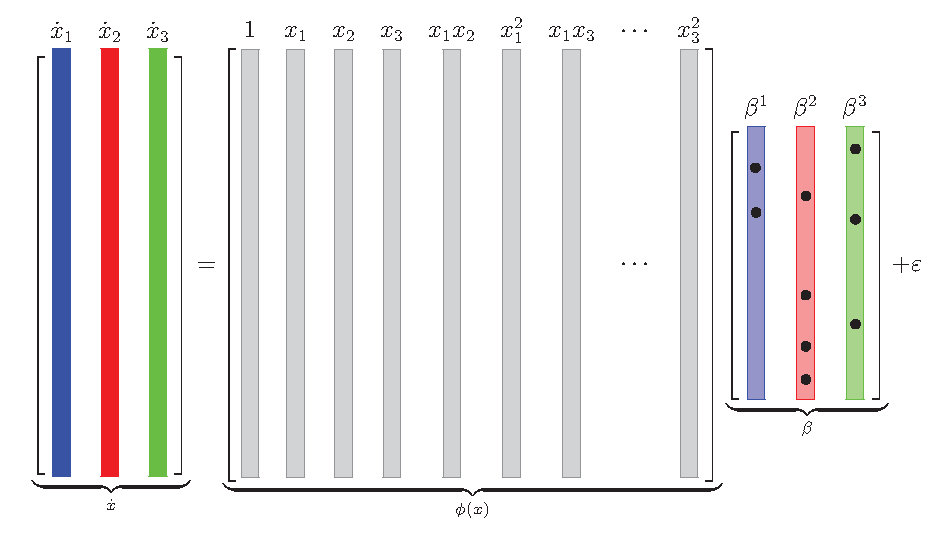
\includegraphics[width=4in]{sindyexplanation}
\end{center}
\vspace{-12pt}
$$
\frac{dx}{dt} = \phi(x) \beta + \varepsilon
$$
\begin{center}
Idea: solve for $\beta$ via sparsity-promoting (least squares) regression.
\end{center}
\end{frame}

\begin{frame}
\frametitle{SINDy (Sparse Identification of Nonlinear Dynamics)}
\begin{block}{More Details}
\begin{itemize}
\item Let $x = (x_1, x_2, \ldots, x_d) \in \mathbb{R}^d$.
\item Suppose there are $N+1$ observations of $x$ and $p$ columns of $\phi(x)$.
\item The $j$-th column of $\phi(x)$ is a function
$$
\phi_j : \mathbb{R}^d \to \mathbb{R}.
$$
\item The user prescribes the $\phi_j$'s.  In the example, we used
polynomial functions of the coordinates; other choices are fine.
\item Reduce problem to finding ``expansion coefficients'' $\beta$:
$$
\frac{dx_i}{dt} = f_i(x) = \sum_{j=1}^p \beta^i_j \phi_j(x) + \varepsilon_i
$$
\end{itemize}
\end{block}
\end{frame}

\begin{frame}
\frametitle{Notation}
Let $\mathcal{N}(\mu, \Sigma)$ denote a multivariate Gaussian/normal in $\mathbb{R}^d$ with:
\begin{itemize}
\item mean vector $\mu \in \mathbb{R}^d$, and
\item $d \times d$ covariance matrix $\Sigma$.
\end{itemize}
\end{frame}

\begin{frame}
\frametitle{Probabilistic Derivation of SINDy}
\begin{block}{Step 1: Discretize in Time}
We return to the SDE
$$
d X_t = f(X_t) dt + \Gamma dW_t.
$$
Assume $\Gamma$ is diagonal.  Discretize in time (for now, using Euler):
$$
\widetilde{X}_{n+1} = \widetilde{X}_n + f(\widetilde{X}_n) h + \Gamma h^{1/2} Z_{n+1}
$$
where $Z_{n+1} \sim \mathcal{N}(0, I)$, independent from $\widetilde{X}_n$.  Note that
$$
[\widetilde{X}_{n+1} | \widetilde{X}_n = v] \sim \mathcal{N}(v + f(v) h, h \Gamma^2).
$$
Now use expansion of $f$ from earlier and assume coefficients are given:
$$
[\widetilde{X}_{n+1} | \widetilde{X}_n = v, \beta] \sim \mathcal{N}(v + \phi(v) \beta h, h \Gamma^2).
$$
\end{block}
\end{frame}

\begin{frame}
\frametitle{Probabilistic Derivation of SINDy}
\begin{block}{Step 2: Markov property}
The overall log likelihood breaks into pieces:
$$
\log p(x_0, x_1, \ldots, x_N | \beta) = \sum_{n=1}^N \log p(x_n | x_{n-1}, \beta)
$$
Identifying $x_n$ with $\widetilde{X}_n$, we can use the Gaussian to write:
\begin{multline*}
\log p(x_0, x_1, \ldots, x_N | \beta) = \sum_{n=1}^N \left[ \sum_{i=1}^d -\frac{1}{2} \log(2 \pi h \gamma_i^2) \right] \\
- \frac{1}{2h} (x_n - x_{n-1} - h \sum_{j=1}^p \phi_j(x_{n-1}) \beta_j)^T \Gamma^{-2} (x_n - x_{n-1} - h \sum_{\ell=1}^p \phi_j(x_{n-1}) \beta_\ell)
\end{multline*}
\end{block}
\end{frame}

\begin{frame}
\frametitle{Probabilistic Derivation of SINDy}
\begin{block}{Step 3: Maximize Likelihood over $\beta$}
Now we set $\Gamma = \sigma I$.  The log likelihood becomes
$$
\log p(x | \beta) = -\frac{N d}{2} \log(2 \pi h \sigma^2) - \frac{1}{2 h \sigma^2} \sum_{n=1}^N \left\| x_n - x_{n-1} - h \sum_{j=1}^p \phi_j(x_{n-1}) \beta_j \right\|_2^2.
$$
Maximizing the log likelihood over $\beta$ is equivalent to minimizing
$$
\sum_{n=1}^N \left\| \frac{x_n - x_{n-1}}{h} - \sum_{j=1}^p \phi_j(x_{n-1}) \beta_j \right\|_2^2.
$$
\textcolor{red}{Except that $dx/dt$ has been discretized in time, this is precisely the same as the SINDy regression problem described above.}
\end{block}
\end{frame}

\begin{frame}
\frametitle{Lessons/Connections Learned}
\begin{itemize}
\item Quality of derivative approximation tied to quality of time-discretization of SDE.
\item SINDy appears to ignore the covariance $\Gamma$ entirely.  I view this as hidden price paid for SINDy's simplicity and scalability.
\item Could return to end of Step 2 and maximize likelihood over both $\beta$ and $\Gamma$.
\item Iterative maximization over $\beta$ and $\Gamma$ in turn is \textcolor{red}{iteratively reweighted least squares} in Statistics.
\end{itemize}
Ongoing/future work: build in priors, sample from posterior $p(\beta | x)$, and thereby quantify uncertainty in $\beta$.
\end{frame}

\begin{frame}
\frametitle{Extending this to SDE}
\begin{block}{Are we done?}
\begin{itemize}
\item We just showed that if we change SINDy slightly and estimate both $\beta$ and $\Gamma$, we've found an SDE model for the data!
\item Caveats:
\begin{enumerate}
\item Quality of approximation is controlled by $h$.

As $h \downarrow 0$, the Euler transition density
$$
\widetilde{x}_{n+1} | \widetilde{x}_n = v
$$
will approach the true transition density of the SDE,
$$
X((n+1) h) | X( n h) = v.
$$
\item When $h$ is small, above small modification to SINDy should work.
\item What $h$ is large, need additional ideas.
\end{enumerate}
\end{itemize}
\end{block}
\end{frame}

\begin{frame}
\frametitle{Large Interobservation Times}
\begin{block}{Idea}
\begin{itemize}
\item Consider data points $\{x_n\}_{n=0}^N$ collected at times $t_n = n \Delta t$.
\item When $\Delta t$ is large, treat the fine scale data as missing data and use expectation maximization (EM).
\item In the ``E'' step, we sample repeatedly from a \textcolor{red}{diffusion bridge} connecting $x_n$ to $x_{n+1}$ on a fine time scale $h$.
\item In this way, we can compute \emph{expected} log likelihoods and then maximize them in the ``M'' step.
\end{itemize}
\end{block}
\end{frame}

\begin{frame}
\frametitle{Concrete Example}
\begin{block}{Noisy Pendulum}
$$
\dot{\mathbf{x}} = \begin{bmatrix} x_2 \\ -\sin x_1 \end{bmatrix} + \Gamma d \mathbf{W}_t
$$
$\Gamma = \operatorname{diag}(.075, .1)$.
$\mathbf{x}(0) = (1,0)$, $\mathbf{x}(T) = (0.927, -0.347)$, and $T = 0.418$. 
Bridges joining the two points with $h = T/1000$:
\begin{center}
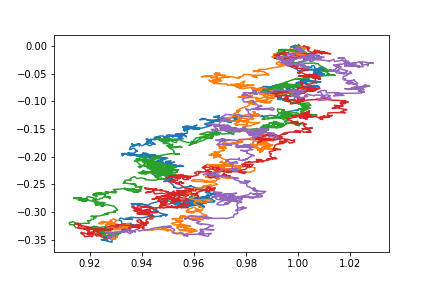
\includegraphics[width=3in]{bridge2d.png}
\end{center}
\end{block}
\end{frame}

\begin{frame}
\frametitle{Expectation Maximization in Detail}
Let $z$ denote the missing fine scale data connecting each $x_{n-1}$ to the next $x_n$.  Then $(x,z)$ is the \emph{completed data} consisting of coarse-scale measurements augmented at a fine scale.
\begin{block}{Algorithm to find parameters $\theta = (\beta,\gamma)$}
\begin{enumerate}
\item Start with an initial guess $\theta^{(0)}$.
\item Define
$$
Q(\theta, \theta^{(k)}) = E_{z | x, \theta^{(k)}} [ \log p(x, z | \theta) ].
$$
\item Maximize $Q$ over $\theta$, i.e., set
$$
\theta^{(k+1)} = \operatorname{argmax}_\theta Q(\theta,\theta^{(k)}).
$$
It will turn out that we can solve this maximization problem without numerical optimization.  (Least squares!)
\end{enumerate}
\end{block}
\end{frame}

\begin{frame}
\frametitle{E-Step}
Let $z^{(r)}$ denote the $r$-th diffusion bridge sample path,
$$
z^{(r)} \sim z | x, \theta^(k).
$$
Let $y = (x,z)$ denote the completed data.  With $R$ bridge samples, we approximate the expected value as follows:
\begin{multline*}
Q(\btheta, \btheta^{(k)}) = \mathbb{E}_{z \mid x, \btheta^{(k)}} [\log p(x, z \mid \btheta)] \approx \frac{1}{R} \sum_{r=1}^R \biggl[ \sum_{j=1}^N \left[ \sum_{i=1}^d -\frac{1}{2} \log (2 \pi h \gamma_i^2) \right] \\
 -\frac{1}{2h} (y_j^{(r)} - y_{j-1}^{(r)} - h \sum_{k=1}^M \phi_k(y_{j-1}^{(r)}) \beta_k )^T \Gamma^{-2} (y_j^{(r)} - y_{j-1}^{(r)} - h \sum_{\ell=1}^M \phi_\ell(y_{j-1}^{(r)}) \beta_\ell ) \biggr]
\end{multline*}
\end{frame}

\begin{frame}
\frametitle{M-Step}
To maximize $Q$ over $\theta$, we first assume $\Gamma$ is known and maximize over $\beta$.  The solution is given by forming the matrix
$$
\mathcal{M}_{k,\ell} = \frac{1}{R} \sum_{r=1}^{R} \sum_{j=1}^N h \phi_k^T (y_{j-1}^{(r)}) \Gamma^{-2} \phi_\ell^T (y_{j-1}^{(r)})
$$
and the vector
$$
\rho_k = \frac{1}{R} \sum_{r=1}^{R} \sum_{j=1}^N \phi_k^T (y_{j-1}^{(r)}) \Gamma^{-2} (y_j^{(r)} - y_{j-1}^{(r)}).
$$
We then solve the system
$$
\mathcal{M} \beta = \rho
$$
for $\beta$.  Now that we have $\beta$, we maximize $Q$ over $\gamma$ and get:
$$
\gamma_i^2 = \frac{1}{R N h} \sum_{r=1}^{R} \sum_{j=1}^N (( y_j^{(r)} - y_{j-1}^{(r)} - h \sum_{\ell=1}^M \beta_\ell \phi_\ell (y_{j-1}^{(r)}) ) \cdot e_i )^2
$$
where $e_i$ is the $i^\text{th}$ canonical basis vector in $\mathbb{R}^d$.
\end{frame}

\begin{frame}
\frametitle{The Above in Plain English}
\begin{itemize}
\item Given coarse data, bridge the data $R$ times.
\item Each time you bridge the data, calculate the regression matrices/vectors \textcolor{red}{that you would've calculated in SINDy.}
\item Now average the $R$ regression matrices/vectors and solve the resulting system for $\beta$.
\item Do the same for $\gamma$.
\end{itemize}
\end{frame}

\begin{frame}
\frametitle{Upshot}
\begin{block}{Properties of EM}
\begin{itemize}
\item Can prove that from one step to the next, the algorithm monotonically increases both $Q$ and the true (incomplete) log likelihood.
\item Hence, starting from guess $\theta^{(0)}$, we use EM to evolve
$$
\theta^{(k+1)} = \operatorname{argmax}_\theta Q(\theta,\theta^{(k)})
$$
Then, as $k \to \infty$,
$$
\theta^{(k)} \to \theta^{\ast},
$$
a local maximizer of the likelihood function.
\end{itemize}
\end{block}
\end{frame}

\begin{frame}
\frametitle{Key Technical Idea}
\begin{block}{MCMC Diffusion Bridge Sampling}
We implement diffusion bridge using MCMC approach that goes back at least to Roberts and Stramer [2001].  Here is the idea:
\begin{itemize}
\item Given $\Gamma$ and two points $(x_0, x_1)$ at times $(0, \Delta t)$, sample from the Brownian bridge process
$$
dY_t = \frac{x_1 - Y_t}{\Delta t - t} dt + \Gamma dW_t
$$
with initial condition $Y_0 = x_0$.  Then $Y_{\Delta t} = x_1$.
\item We treat this sample as a proposal, \textcolor{red}{$Z_t^\ast$}.  Suppose the previous MCMC bridge was \textcolor{red}{$Z_t^\text{old}$}.
\end{itemize}
\end{block}
\end{frame}

\begin{frame}
\frametitle{Key Technical Idea}
\begin{block}{MCMC Diffusion Bridge Sampling}
\begin{itemize}
\item By Girsanov's theorem, the Metropolis accept probability is
$$
\min \left\{1, \frac{\psi(Z_t^\ast)}{\psi(Z_t^\text{old})} \right\}
$$
with
$$
\log \psi(z) = \Gamma^{-2} \underbrace{\int_0^{\Delta t} f(Z_s) dZ_s}_\text{stochastic} - \frac{1}{2} \Gamma^{-2} \underbrace{\int_0^{\Delta t} f(Z_s)^2 \, ds}_\text{ordinary}.
$$
\item Both the stochastic and ordinary integrals can be easily evaluated numerically.
\item In practice, we obtain reasonable acceptance rates in this way.
\end{itemize}
\end{block}
\end{frame}

\begin{frame}
\frametitle{Ongoing/Future Work}
Preliminary results are promising!  We plan to submit to NIPS '18.\smallskip
\begin{itemize}
\item Testing the EM+bridge approach on stochastic versions of nonlinear dynamical systems in $d=3$.
\item Quantifying relationship between magnitude of noise and quality of reconstruction.
\item Applying these techniques to real data.
\item Comparing against competing approaches.
\end{itemize}
Email me at hbhat@ucmerced.edu if you'd like any notes or code on this.\bigskip

Support from NSF DMS-1723272 gratefully acknowledged.
\end{frame}

\end{document}


